\chapter{Methodology}

\section{Algorithms}

We have modified the \ac{A3C} algorithm in order to take advantage of sub-tasks with the purpose of enhancing training speed
and exploration.
We refer to this new algorithm as \acf{MA3C} and in this section it can be found specifications about the architectures of
both \acp{ANN}: \ac{A3C} and \ac{MA3C}.
In addition we will explain the \ac{MA3C} algorithm.

They have been developed using tensorflow (\cite{tensorflow2015}), an open source machine learning framework which the authors
of \ac{A3C} and \ac{DQN} are also using (\cite{deepmind_tensorflow}).

\subsection{\acl{A3C}\label{subsec:AlgorithmA3C}}

As we have explained before (\ffref{subsec:A3C}), this algorithm uses the image of the environment to represent the state.
We have used almost the same preprocessing and network architecture (\ffref{fig:A3C}) than in \citetitle{mnih2016A3C} (\cite{mnih2016A3C}).
In practice, the images of any game are resized to $84 \times 84$ greyscale pixels in order to reduce the computational cost of training,
specifically the input dimensionality, and also to fit the convolutions.
The algorithm applies this preprocessing to 4 stacked frames allowing the \ac{ANN} to implicitly calculate the movement
of the different pixels/objects on the screen.
There is a frame skip of 4, which means that, only one out of four consecutive frames is taken into account and stacked.
There is also a component-wise maximum selection over two consecutive frames, the one stacked and the next one which will
not be stacked.
The state dimensionality is $84 \times 84 \times 4$ which defines the input layer of the \ac{CNN}.
This is just for Atari games, in Simple States (\ffref{subsec:SimpleStates}) and Complex States (\ffref{subsec:ComplexStates})
the RGB channels of a single frame are used instead.
The dimensionality of the input layer in that games is $84 \times 84 \times 3$.

There are several hidden layers specifically designed to obtain high level abstractions of the environment frames.
The first one is a convolutional layer (\ffref{subsec:CNN}) with $16$ filters with kernel dimension $8 \times 8$ and stride $4$,
followed by a \ac{ReLU} layer.
The second layer is also a convolutional layer, but with $32$ filters with kernel dimension $4 \times 4$ and stride 2,
again followed by a \ac{ReLU} layer.
The last hidden layer intends to represent general features about the state of the game.
It is a fully connected composed by 256 ReLU nodes.

From these 256 features the actor and critic layers, which are the output layers, decide the actions that should be taken
in order to maximize the reward, as explained in (\ffref{subsec:AC}).
The actor is made up by as many nodes as actions available in each game with values from $0$ to $1$, representing the
probability distribution $\pi$.
The critic is just $1$ neuron representing the value function $V(s_t)$.

\begin{figure}[hbtp]
\begin{center}
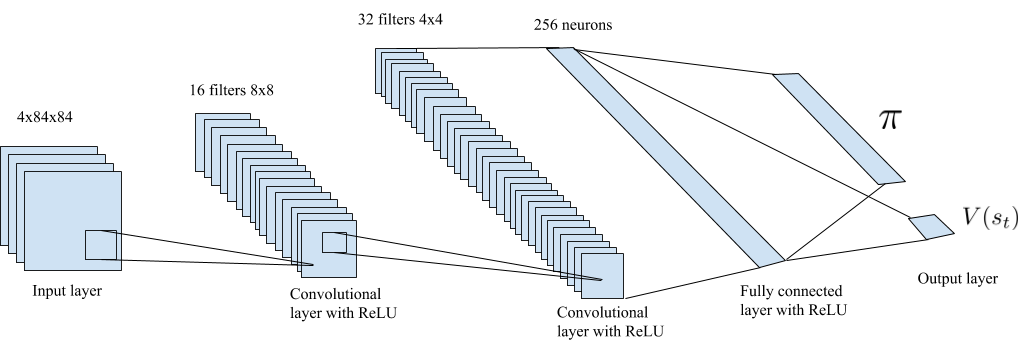
\includegraphics[width=430]{img/A3C_architecture.png}
\end{center}
\caption[A3C architecture]
{Architecture of the \ac{A3C} algorithm.}
\label{fig:A3C}
\end{figure}

\subsection{\acl{MA3C}\label{subsec:MA3C}}

This algorithm is strongly associated with hierarchial reinforcement learning, since the last layer of \ac{A3C}
($\pi$ and $V(s_t)$) is replicated several times in order to model different tasks inside a common bigger problem.

\begin{figure}[hbtp]
\begin{center}
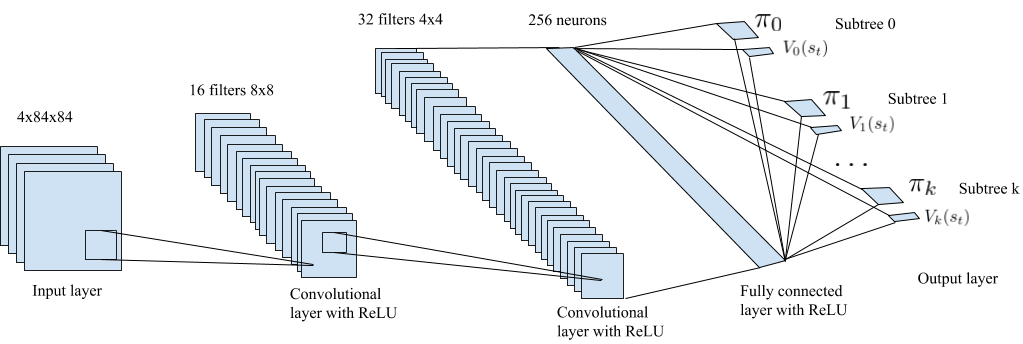
\includegraphics[width=430]{img/MA3C_architecture.png}
\end{center}
\caption[MA3C architecture]
{Architecture of the \ac{MA3C} algorithm.}
\label{fig:MA3C}
\end{figure}

As we can see in \ffref{fig:MA3C} the architecture is very similar to \ac{A3C}.
There is an input layer of size $84 \times 84 \times 4$, a convolutional layer with $16\; 8 \times 8$ filters, another
convolutional layer with $32 \; 4 \times 4$ filters and a fully connected layer with $256$ nodes.
The output layer is made up by $K$ copies of the \ac{A3C} output layer, where $K = k-1$ is an hyperparameter which might be
different depending on the use case.
For each of the games we have set $K$ to a different value: with Simple States we have used $K=3$, with Complex States
$K=2$ and with \ac{MR} $K=4$.
The first two depend on the number of phases (see \ffref{subsec:SimpleStates} and \ffref{subsec:ComplexStates}) and the last one
depends on the number of intermediate rewards (see \ffref{subsec:MontezumasRevenge}).

The architecture of \ac{MA3C} contains multiple \newconcept{subtrees} defining different \acl{AC} approaches to the given input state,
each one connected to the high level features (last layer) but not between them.
With this architecture the algorithm uses transfer learning (\ffref{subsec:TransferLearning}) to extract common features
about the environment, which are useful for all \ac{AC} layers.
When some task is already trained and a new one starts to train, most of the network is reused, speeding up the learning
process.
Given that every subtree is used to solve a different task inside a bigger problem, the common parameters will be optimized to
extract as much information as possible about the general problem, while the weights of each subtree will be optimized to
succeed in the specific task.

The update function, advantage function and algorithm of \ac{MA3C} remain the same ones as in \ac{A3C} (\ffref{subsec:A3C}).
The only difference is that this one selects the chunk of the parameter vectors $\theta'$ and $\theta_{v}'$ that will be updated
depending on the currently active subtree.
The method which selects one subtree or another is arbitrary, they might be selected with an \ac{AI} method, just
with a couple of rules or be given by the state.
For this thesis we have used two approaches: part of the state, in Simple States (\ffref{subsec:SimpleStates}) and Complex States
(\ffref{subsec:ComplexStates}); and some rules about the position of the hero in Montezuma's Revenge (\ffref{subsec:MontezumasRevenge}).

The full modified algorithm is shown in \ffref{alg:MA3C}.

\begin{algorithm}[hbtp]
\begin{algorithmic}
    \State \newconcept{//Assume global shared parameter vectors $\theta$ and $\theta_v$ and global shared counter $T = 0$}
    \State \newconcept{//Assume thread-specific parameter vectors $\theta' and \theta_v'$}
    \State \newconcept{//Assume subree-specific parameter vectors $\theta'^k and \theta_v'^k$ from $\theta' and \theta_v'$}
    \State Initialize thread step counter $t \leftarrow 1$
    \Repeat
        \State Reset gradients: $d\theta \leftarrow 0$ and $d\theta_v \leftarrow 0$.
        \State Synchronize thread-specific parameters $\theta' = \theta$ and $\theta_v' = \theta_v$
        \State $t_{start} = t$
        \State Get state $s_t$
        \Repeat
            \State Perform $a_t$ according to policy $\pi(a_t|s_t;\theta')$
            \State Receive reward $r_t$ and new state $s_{t+1}$
            \State $t \leftarrow t + 1$
            \State $T \leftarrow T + 1$
        \Until{terminal $s_t $ \textbf{or} $t-t_{start} == t_{max}$ }
        \State R = \begin{cases}
                0,   & \text{ for terminal }\ s_t \\
                V(s_t, \theta_v'),   & \text{for non-terminal } s_t \;\newconcept{// Bootstrap from last state}\\
            \end{cases}
        \For{ $i \in \{ t-1,\dots,t_{start}\}$}
            \State $R \leftarrow r_i + \gamma R$
            \State Select $k$ \;\newconcept{// Select subtree with any criteria}
            \State Accumulate gradients wrt $\theta'^k: d\theta \leftarrow d\theta + \nabla_{\theta'} log\:\pi(a_i\mid s_i;\theta')(R-V(s_i;\theta_v'))+\beta\nabla_{\theta'}H(\pi(s_i;\theta'))$
            \State Accumulate gradients wrt $\theta_v'^k: d\theta_v \leftarrow d\theta_v + \partial(R-V(s_i;\theta_v'))^2 / \partial \theta_{v}'$
        \EndFor
        \State Perform asynchronous update of $\theta$ using $d\theta$ and of $\theta_v$ using $d\theta_v$.
    \Until{$T > T_{max}$}
\end{algorithmic}
\caption{\acl{MA3C} - psudocode for each actor-learner thread (\cite{mnih2016A3C})}
\label{alg:MA3C}
\end{algorithm}

\section{Environments}

In order to demonstrate the capabilities of \ac{MA3C} over \ac{A3C} we have developed two simple environments where the
weaknesses of the second one come to light.
We have also compared the algorithms in a real game, \acl{MR}, which has become famous because of its difficulty.

These three environments have been used through a useful toolkit called OpenAi Gym (\cite{gym}), in which the different games
can be accessed by a common interface facilitating the analysis of different algorithms and games.


\subsection{Simple States\label{subsec:SimpleStates}}

This game is made by a $6 \times 10$ grid of square blocks.
Their colors define the kind of object and how they will interact with the hero (an special object).
This are the different types:
\begin{itemize}
  \item \newconcept{hero}: A block that can be controlled by the actions.
  \item \newconcept{wall}: If the hero hits a wall the game ends and he obtains a reward of value -1.
  When this happens we say that the hero dies.
  \item \newconcept{checkpoint}: When the hero reach this object he obtains a reward of value 1 and enables the hidden
  checkpoint reward.
  Once the hero reaches it for the first time he will never obtain the reward again.
  \item \newconcept{hidden checkpoint}: When the hero reach this object enables the door.
  It basically forces the hero to pass and there is no reward when this happens.
  \item \newconcept{door}: If the hero reach the door having gone through the different checkpoints the game ends and
  he obtains a reward of value 1.
\end{itemize}

\begin{figure}[hbtp]
\begin{center}
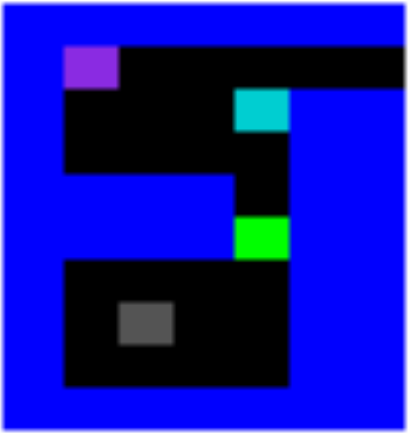
\includegraphics[width=200]{img/SimpleStates_going_up.png}
\end{center}
\caption[Simple States game]
{The hero navigating through a hostile environment trying to reach the door. The wall, hero, checkpoint, hidden checkpoint
and door are represented with the following colors respectively: blue, grey, green, turquoise and violet.}
\label{fig:SimpleStates}
\end{figure}

The goal of the hero is to reach the door by passing through the different checkpoints without colliding
with any wall, this will give to the hero the maximum score, 2 points.
The game is organized in three different phases/states, each one having a different objective.
The first one's objective is to reach the checkpoint,
of the second one's, the hidden checkpoint and the third one's, the door.
The information about the current phase is allways available to the player.

In order to solve this game with both \ac{A3C} and \ac{MA3C} algorithms we must model it as a \ac{SMDP} problem,
describing components of the tuple $\langle\mathcal{S}, \mathcal{A}_s, \mathcal{P}_a(s,s'), \mathcal{R}_a(s,s'), \gamma \rangle$.

\begin{itemize}
    \item Each states is a pair $s_t = (\mathbf{F}, p)$ where $p \in \{0,1,2\}$ is the phase of the game and
    $\mathbf{F}$ is the matrix of RGB pixels with dimensionality $84\times84\times3$.
    $\mathcal{S}$ is the set of all $s$ which satisfies the conditions about object collisions presented above.

    \item $\forall s \; \mathcal{A}_s = \{\textsc{UP}, \textsc{DOWN}, \textsc{LEFT}, \textsc{RIGHT}, \textsc{WAIT}\}$ and each action $a_{t}\in \mathcal{A}_s $ corresponds to
    the movement of the hero.

    \item This game is deterministic, which means that $\forall s\forall a\exists s' \; |\; \mathcal{P}_a(s,s') = 1$ implying
    $\forall s\forall a\forall {s''\neq s'} \;\; \mathcal{P}_a(s,s'') = 0$

    \item The reward function is determined as explained before.
    Depending on the phase ($p$) some transition from a frame $\mathbf{F}_t$
    to another frame $\mathbf{F}_{t+1}$ may come with a reward $\mathcal{R} \in \{ -1, 0, 1\}$.

    \item The discount factor $\gamma$ is $0.99$
\end{itemize}

The purpose of creating this game is to prove that the \ac{MA3C} algorithm (\ffref{subsec:MA3C}) has better exploration
skills than A3C (\ffref{subsec:A3C}).

% TODO F PONER QUE CUMPLE LA MARKOV PROPERTY?
\subsection{Complex States\label{subsec:ComplexStates}}

This game is really similar to the previous one but the dynamics are a bit different.
The hero must follow a series of steps to reach the door.
The order in which the hero must go through the objects is: checkpoint $\rightarrow$ hidden checkpoint $\rightarrow$
door $\rightarrow$ hidden checkpoint $\rightarrow$ checkpoint $\rightarrow$ door.
We force the hero to go back on his own steps when he reaches the door.
In this game some of the rewards also change.
These are the changes with respect to the Simple States game, the rest remains equal:
\begin{itemize}
    \item \newconcept{checkpoint}: The first time that the hero goes through this object he obtains a reward of 1.
    Then he must follow the rest of the path described above to obtain again 1 of score (after the second time he visits the hidden checkpoint).
    \item \newconcept{hidden checkpoint}: In this game both 2 times that the hero goes through this object
    (following the path) receives 1 of score.
    The first time the checkpoint object enables the reward and the second time the door enables it.
    \item \newconcept{door}: The first time the hero reach the door it moves to the starting position of the hero (bottom left corner)
    and gives him 1 of score.
    The second time behaves as in Simple States.
\end{itemize}

\begin{figure}[hbtp]
\begin{center}
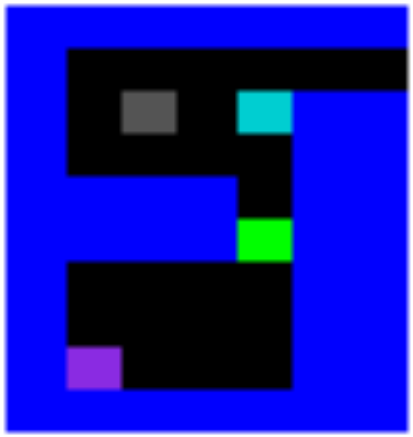
\includegraphics[width=200]{img/ComplexStates_going_back.png}
\end{center}
\caption[Complex States game]
{The hero after reaching the door for first time. The wall, hero, checkpoint, hidden checkpoint
and door are represented with the following colors respectively: blue, grey, green, turquoise and violet.}
\label{fig:ComplexStates}
\end{figure}


In this game there are only two phases.
The first one goes from the start until the first time the hero reaches the door.
The second one finishes the second time it reaches the door.
As in Simple States the hero must follow the path in order to obtain the rewards and finish the game.
The information about the current phase is also available to the player.

The \ac{MDP} problem of this game is exactly the same as in Simple States (\ffref{subsec:SimpleStates}).
The only thing that changes are the rules of rewards and phases which we have already defined.

The purpose of creating this game is to prove that \ac{A3C} is quite bad going back on his own steps (when the image of the
game is similar) while for \ac{MA3C} is easy.

\subsection{Montezuma's Revenge\label{subsec:MontezumasRevenge}}

We wanted to test \ac{MA3C} in an environment which other authors also did a research on.
\acf{MR} is an Atari game created in 1984 which recently has become famous because of its difficulty.
\ac{DQN} and \ac{A3C} algorithms get less than $100$ score on average when playing this game (\cite{mnih2016A3C}).

The hero, Panama Joe, goes into an Aztec pyramid full of treasures, traps and monsters.
The game takes place inside the pyramid where there are different rooms with the treasures he must collect.
In order to navigate from a room to another he must collect keys and open doors while avoiding traps and monsters.
It is a relatively big game (24 rooms) where the agent starts in screen 1 (\ffref{fig:MontezumasRevenge}) and must navigate
through most of the rooms in order to collect a group of special gems which make him win the game.

\begin{figure}[hbtp]
\begin{center}
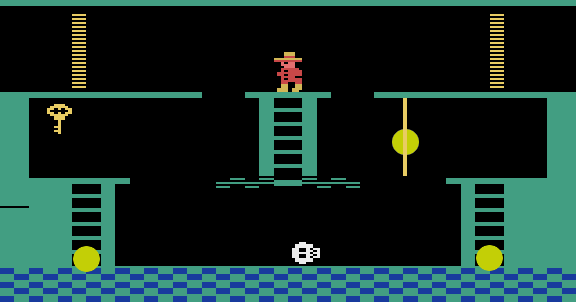
\includegraphics[width=300]{img/montezuma_checkpoints.png}
\end{center}
\caption[Montezuma's Revenge game]
{The hero is in the starting position of the game, in the first screen of \acl{MR}.
Three yellow bullets have been added in order to represent the checkpoints.}
\label{fig:MontezumasRevenge}
\end{figure}

Since this game is really complex and computationally expensive to train, we have made some changes to it.
\begin{itemize}
    \item In the hole game there are several screens but we will only use the first one in my experiments.
    \item The hero has multiple lives but we will consider he has just $1$ and, if he dies, the game will be reset.
    \item When the hero reaches the key we will also reset the game, so the unique goal of the hero is to take that object.
\end{itemize}
Nevertheless, the procedures remain the same as in the original game.

At each time step, the player can take 8 different actions: \textsc{Noop} (stay
still), \textsc{Fire} (jump straight up), \textsc{Up}, \textsc{Right},
\textsc{Left}, \textsc{Down}, \textsc{LeftFire} (jump to the left),
\textsc{RightFire}.

There are one rope and three stairs with which the hero can go up and down.
If he jumps into the rope he will grab it, not as with stairs. %TODO No se entiende la ultima frase
From now on we will refer to the right stairs as \newconcept{Rstairs} and to left ones \newconcept{Lstairs}.
We will use later the position (in screen space) of the objects, which are the following:
\begin{itemize}
    \item rope: from $(109, 174)$ to $(109, 212)$
    \item Rstairs: $(133, 148)$
    \item Lstairs: $(21, 148)$
    \item key: $(14, 209)$
\end{itemize}
In order to obtain this positions, and the agent's position, we have used the memory layout described in \citetitle{adriaTFG}
(\cite{adriaTFG}).

The hero can die within two manners: by falling into the floor from some high position (e.g. from the rope) or by touching the skull in the bottom, which is always moving left and right. %TODO siempre que quieras poner por ejemplo usa e.g. (busca lo que son e.g. y i.e. y usalos siempre)

The hero can obtain a score by collecting the key, which gives him 100 points.
He can also win 10 points by passing through each of the checkpoints which we have manually added to guide the agent
towards the key.
Since they have been selected in order to guide the agent towards $\pi^*$ this is a way of applying reward shaping
(\ffref{subsec:RewardShaping}) to Montezuma's Revenge.
The potential function $\phi(s)$ is defined in the following way:
\begin{equation}
    \State \phi(s) = \begin{cases}
                 10, & \text{hero visits for the first time the positions: rope, Rstairs, Lstairs, key} \\
                 0,  & \text{otherwise} \\
            \end{cases}
\end{equation}

The difficulty is due to the facility to die and the remoteness of the rewards.

We have modeled this game as a \ac{SMDP} (\ffref{subsec:SMDP}),
with the tuple $\left< \mathcal{S}, \mathcal{O}_s, P_o(s,s'), R_o(s),\gamma \right>$.

The state $s \in \mathcal{S}$ is a pair $s_t = (\mathbf{F}, p)$ where $p \in \{0,1,2,3\}$ is the phase/option of the game and
$\mathbf{F}$ is the matrix of processed pixels (as described in \ffref{subsec:AlgorithmA3C}).

The different phases are described by consecutive options in which $\mathcal{I}$ and $\beta$ are specified, but $\pi$
must be learned by the algorithm.
The consecutive options, in order of appearance, are the following:
\begin{itemize}
    \item $o_0$ is the option defined by $\mathcal{I} = {s_0}$, the game initial state, and
    $\beta$ being:
    \begin{equation}
    \State \beta = \begin{cases}
                 1, & \forall s \in \mathcal{S}_{rope} \\
                 0,  & \forall s \notin \mathcal{S}_{rope} \\
            \end{cases}
    \end{equation}
    Where $\mathcal{S}_{rope}$ is the set of states in which the agent is in the same screen space as the rope.

    \item $o_1$ is the option defined by $\mathcal{I} = \mathcal{S}_{rope}$ and
    $\beta$ being:
    \begin{equation}
    \State \beta = \begin{cases}
                 1, & \forall s \in \mathcal{S}_{Rstairs} \\
                 0,  & \forall s \notin \mathcal{S}_{Rstairs} \\
            \end{cases}
    \end{equation}
    Where $\mathcal{S}_{Rstairs}$ is the set of states in which the agent is in the same screen space as the Rstairs.

    \item $o_2$ is the option defined by $\mathcal{I} = \mathcal{S}_{Rstairs}$ and
    $\beta$ being:
    \begin{equation}
    \State \beta = \begin{cases}
                 1, & \forall s \in \mathcal{S}_{Lstairs} \\
                 0,  & \forall s \notin \mathcal{S}_{Lstairs} \\
            \end{cases}
    \end{equation}
    Where $\mathcal{S}_{Lstairs}$ is the set of states in which the agent is in the same screen space as the Lstairs.

    \item $o_3$ is the option defined by $\mathcal{I} = \mathcal{S}_{Lstairs}$ and
    $\beta$ being:
    \begin{equation}
    \State \beta = \begin{cases}
                 1, & \forall s \in \mathcal{S}_{key} \\
                 0,  & \forall s \notin \mathcal{S}_{key} \\
            \end{cases}
    \end{equation}
    Where $\mathcal{S}_{key}$ is the set of states in which the agent is in the same screen space as the rope.
    Bear in mind that $\beta$ is defined in a way that the option finishes in the same states as the game does.
\end{itemize}
The action set available inside each option is
$\mathcal{A}_s = \{\textsc{Noop}, \textsc{Fire}, \textsc{Up}, \textsc{Right}, \textsc{Left},$
$\textsc{Down}, \textsc{LeftFire}, \textsc{RightFire}\}$.
By defining the options in this way, we divide the problem in 4 phases from which, once
it changes to the next, it is impossible to go back to another previous option/phase.
This simplifies the game, being really similar to Simple States and Complex States games.

%TODO EL K DE AQUI ES DISTINTO AL DE MA3C
As far as the agent will learn how to act inside the option, we cannot accurately define $ P_o(s,s') $ and $ R_o(s) $.
This is because the number of steps $k$ depends on the policy of the option.
But we can say that options $o_0, o_1$ and $o_2$ have a reward $r_{t+k} = 10$ while $o_3$ has a reward $r_{t+k} = 110$,
that is, the score given by the key and by the checkpoint.

The discount factor $\gamma$ is $0.99$.

We have decided to model this problem as a \ac{SMDP} in order to expose the strengths of \ac{MA3C} inside hierarchical
learning models, in the knowledge that modeling it as a \ac{MDP} may have been easier and makes more sense.


%%% Local Variables: 
%%% mode: latex
%%% TeX-master: "../report"
%%% End: 
